\begin{frame}{Dynamic Dispatching}
    \begin{itemize}
        \item When designing a system you usually know which kind of interface
            do you want but not the concrete implementation
        \item The goal is to reduce the effort in changing implementations
        \item \textbf{Dynamic Dispatching:} Which mplementation of a 
            method(class function) to call at run-time
    \end{itemize}
\end{frame}

\begin{frame}{Virtual Functions}
    \begin{center}
        \begin{tikzpicture}[]
            \node[] at (0mm,0mm){
                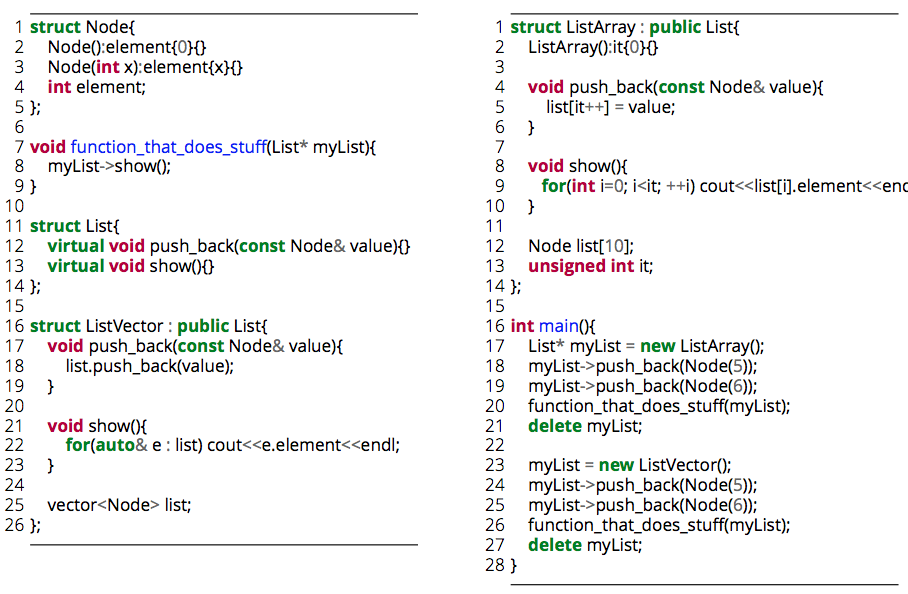
\includegraphics[height=70mm]{/Users/lalanne/MyCode/GitHubProjects/MetaTalk/figures/ddp1.png}\hspace{5mm}
            };
        \end{tikzpicture}
    \end{center}
\end{frame}

\begin{frame}{Virtual Functions}
    \begin{center}
        \begin{tikzpicture}[]
            \node[] at (0mm,0mm){
                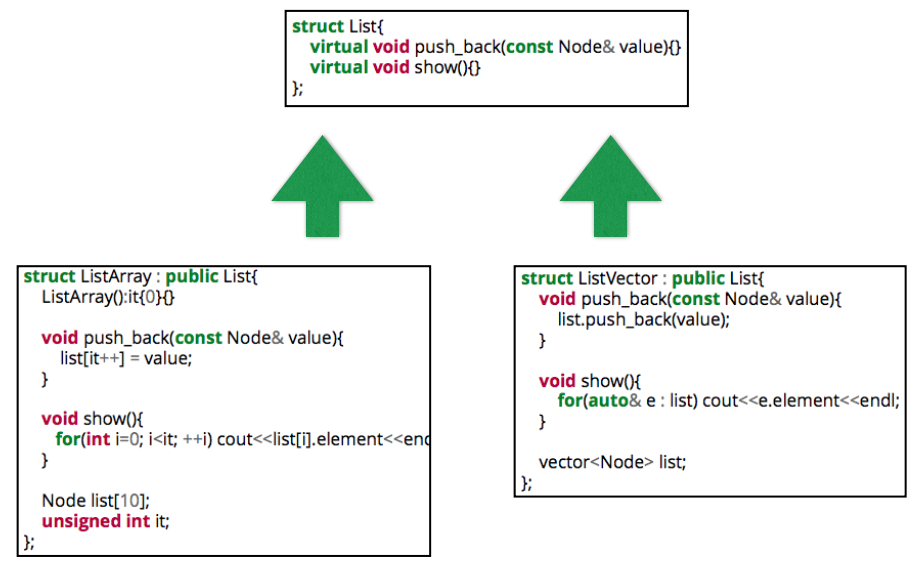
\includegraphics[height=70mm]{/Users/lalanne/MyCode/GitHubProjects/MetaTalk/figures/classdiag.png}\hspace{5mm}
            };
        \end{tikzpicture}
    \end{center}
\end{frame}

\begin{frame}{Virtual Functions}
    \begin{center}
        \begin{tikzpicture}[]
            \node[] at (0mm,0mm){
                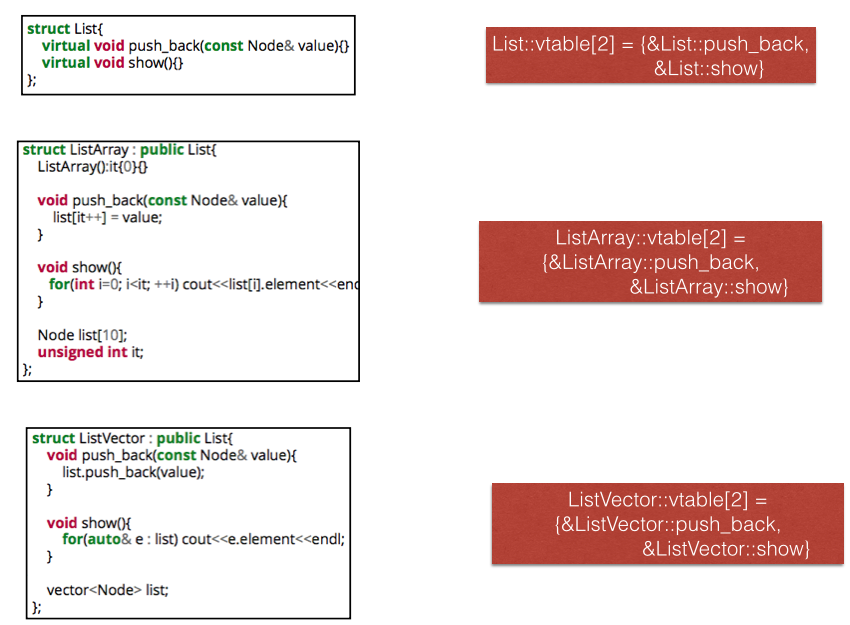
\includegraphics[height=70mm]{/Users/lalanne/MyCode/GitHubProjects/MetaTalk/figures/vtbl1.png}\hspace{5mm}
            };
        \end{tikzpicture}
    \end{center}
\end{frame}

\begin{frame}{Virtual Functions}
    \begin{center}
        \begin{tikzpicture}[]
            \node[] at (0mm,0mm){
                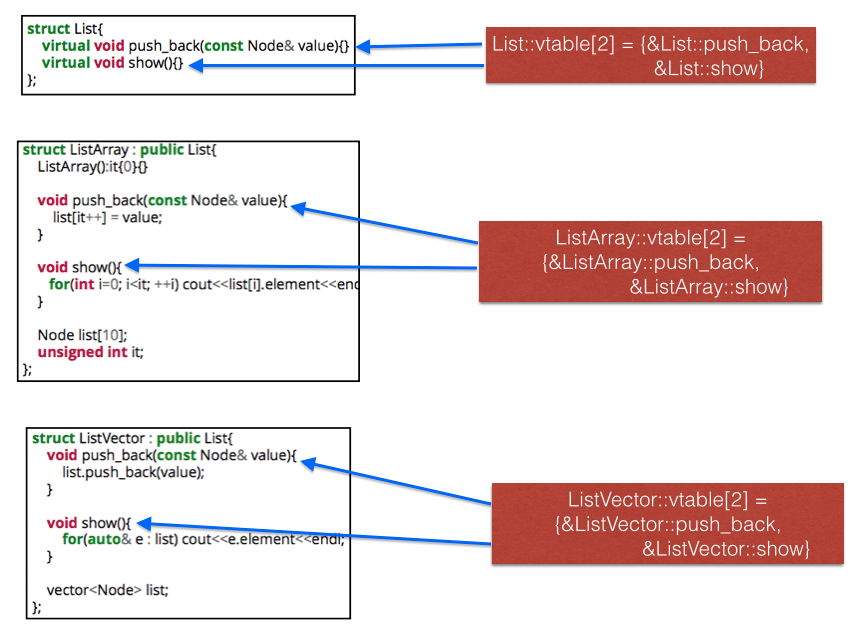
\includegraphics[height=70mm]{/Users/lalanne/MyCode/GitHubProjects/MetaTalk/figures/vtbl1_1.png}\hspace{5mm}
            };
        \end{tikzpicture}
    \end{center}
\end{frame}

\begin{frame}{Virtual Functions}
    \begin{center}
        \begin{tikzpicture}[]
            \node[] at (0mm,0mm){
                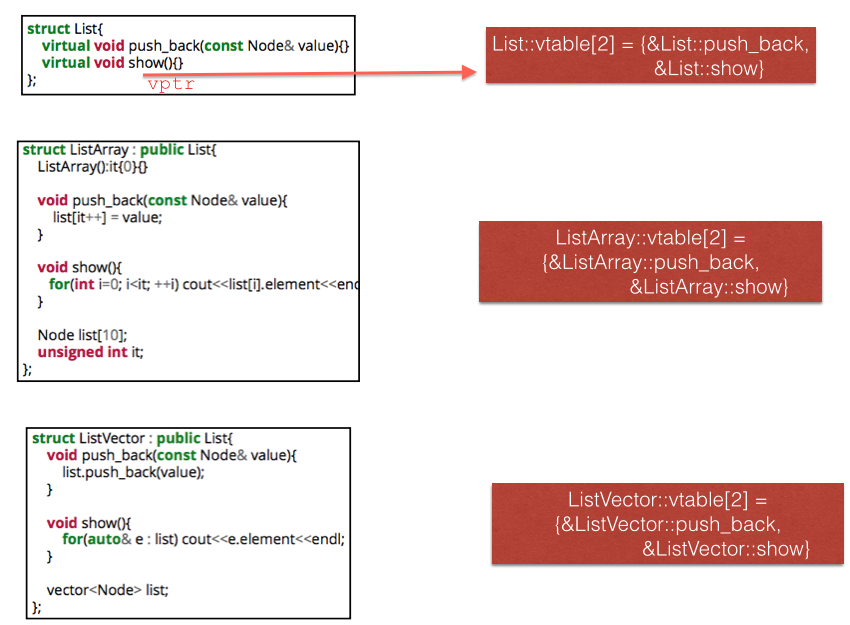
\includegraphics[height=70mm]{/Users/lalanne/MyCode/GitHubProjects/MetaTalk/figures/vtbl2.png}\hspace{5mm}
            };
        \end{tikzpicture}
    \end{center}
\end{frame}

\begin{frame}{Virtual Functions}
    \begin{center}
        \begin{tikzpicture}[]
            \node[] at (0mm,0mm){
                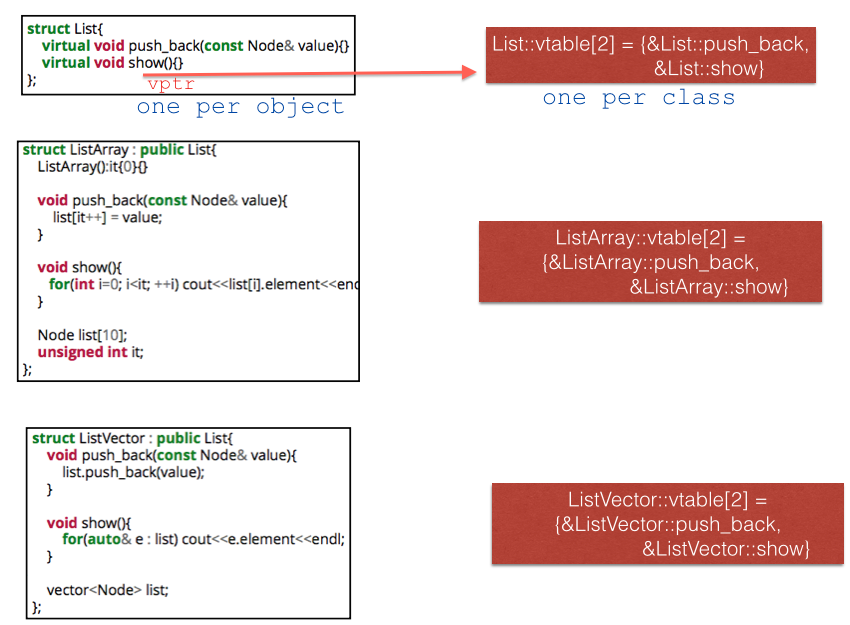
\includegraphics[height=70mm]{/Users/lalanne/MyCode/GitHubProjects/MetaTalk/figures/vtbl3.png}\hspace{5mm}
            };
        \end{tikzpicture}
    \end{center}
\end{frame}

\begin{frame}{Virtual Functions}
    \begin{center}
        \begin{tikzpicture}[]
            \node[] at (0mm,0mm){
                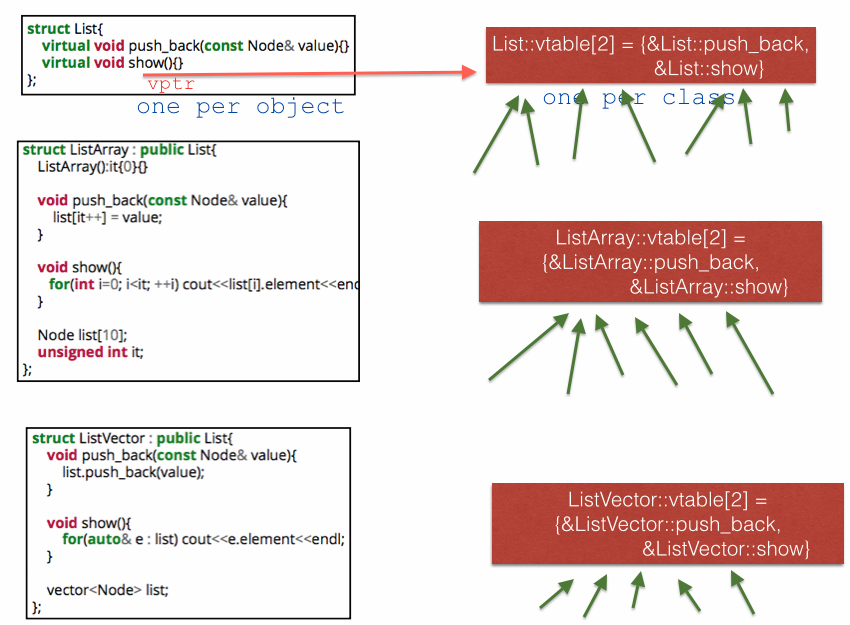
\includegraphics[height=70mm]{/Users/lalanne/MyCode/GitHubProjects/MetaTalk/figures/vtbl3_1.png}\hspace{5mm}
            };
        \end{tikzpicture}
    \end{center}
\end{frame}

\begin{frame}{Virtual Functions}
    \begin{center}
        \begin{tikzpicture}[]
            \node[] at (0mm,0mm){
                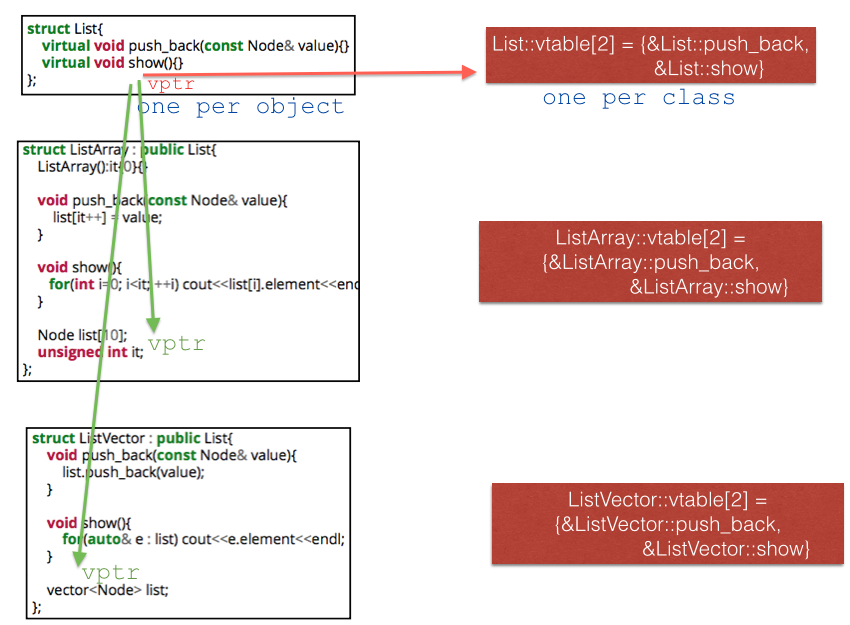
\includegraphics[height=70mm]{/Users/lalanne/MyCode/GitHubProjects/MetaTalk/figures/vtbl4.png}\hspace{5mm}
            };
        \end{tikzpicture}
    \end{center}
\end{frame}


\begin{frame}{Virtual Functions}
    \begin{center}
        \begin{tikzpicture}[]
            \node[] at (0mm,0mm){
                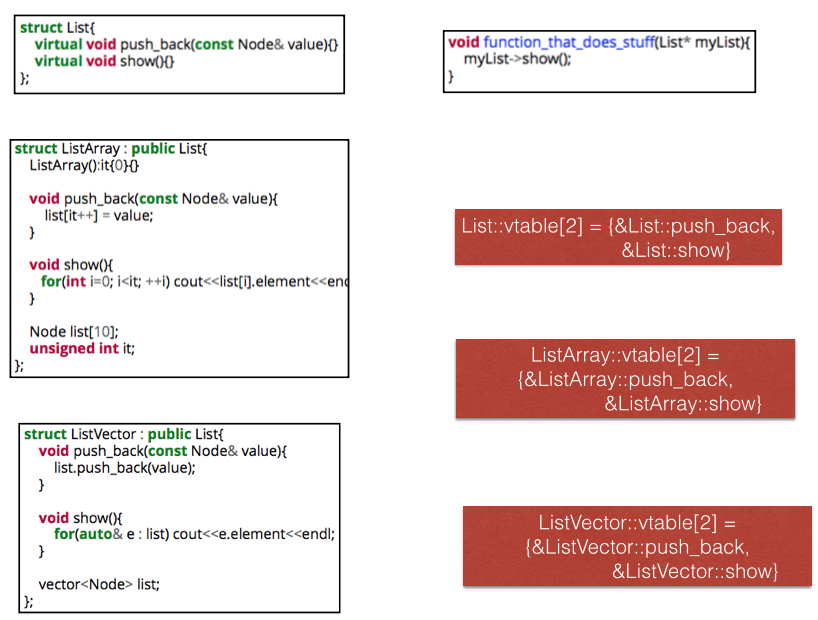
\includegraphics[height=70mm]{/Users/lalanne/MyCode/GitHubProjects/MetaTalk/figures/vtblpluscall.png}\hspace{5mm}
            };
        \end{tikzpicture}
    \end{center}
\end{frame}

\begin{frame}{Virtual Functions}
    \begin{center}
        \begin{tikzpicture}[]
            \node[] at (0mm,0mm){
                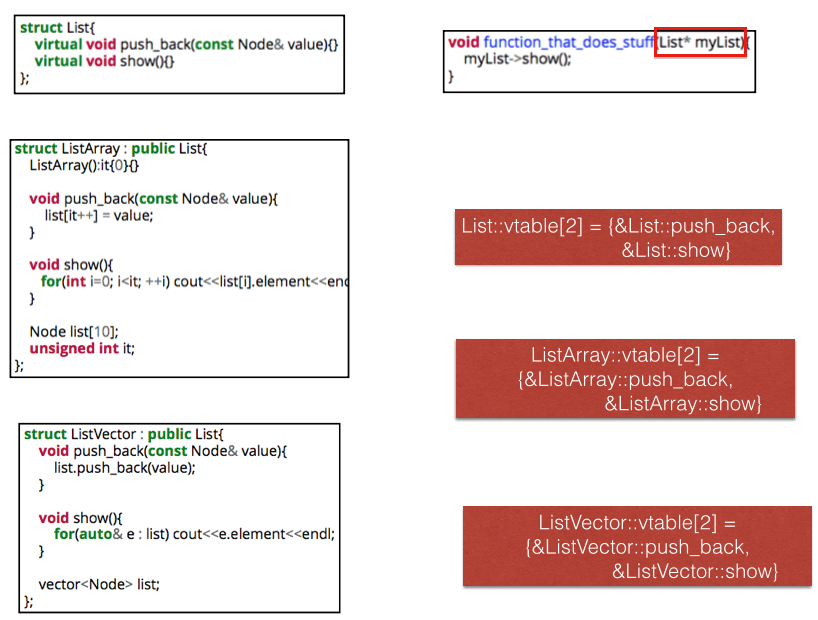
\includegraphics[height=70mm]{/Users/lalanne/MyCode/GitHubProjects/MetaTalk/figures/vtblpluscall1.png}\hspace{5mm}
            };
        \end{tikzpicture}
    \end{center}
\end{frame}

\begin{frame}{Virtual Functions}
    \begin{center}
        \begin{tikzpicture}[]
            \node[] at (0mm,0mm){
                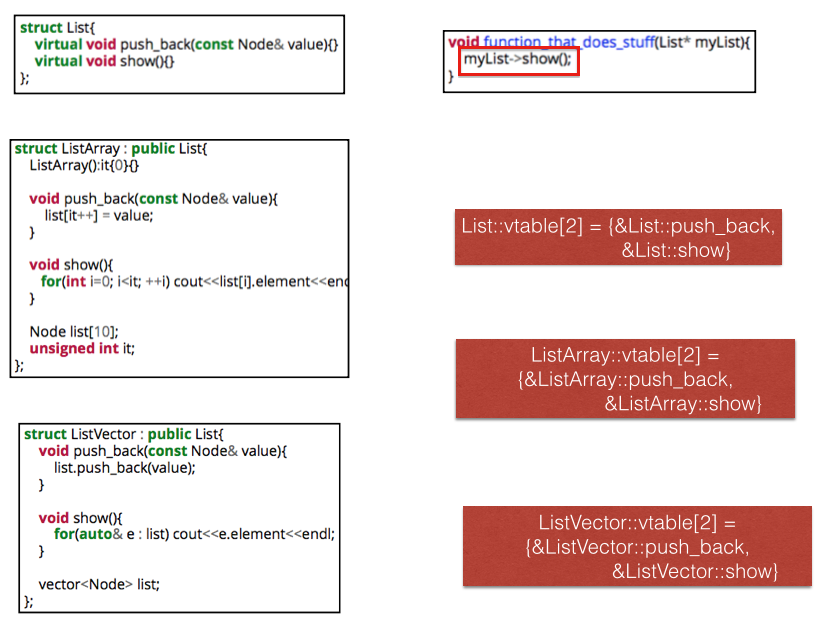
\includegraphics[height=70mm]{/Users/lalanne/MyCode/GitHubProjects/MetaTalk/figures/vtblpluscall2.png}\hspace{5mm}
            };
        \end{tikzpicture}
    \end{center}
\end{frame}

\begin{frame}{Virtual Functions}
    \begin{center}
        \begin{tikzpicture}[]
            \node[] at (0mm,0mm){
                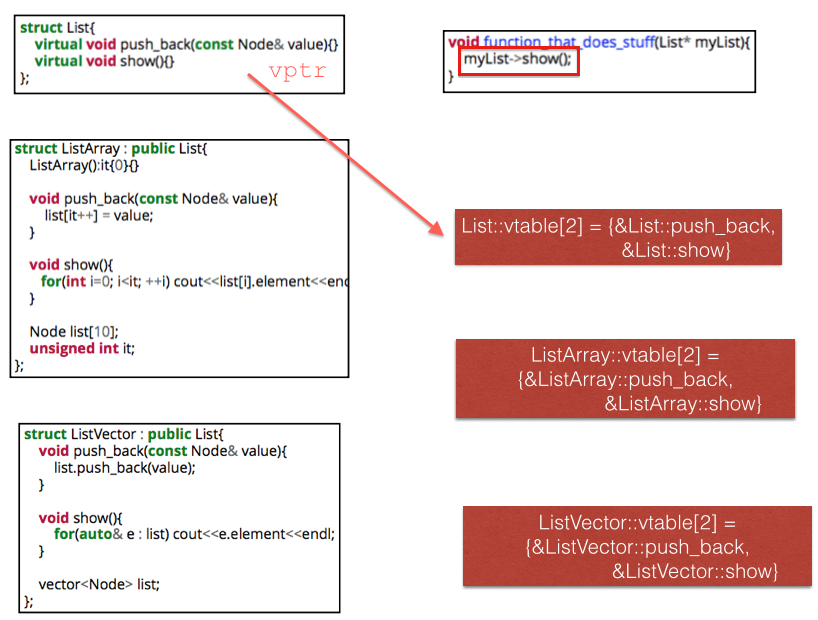
\includegraphics[height=70mm]{/Users/lalanne/MyCode/GitHubProjects/MetaTalk/figures/vtblpluscall3.png}\hspace{5mm}
            };
        \end{tikzpicture}
    \end{center}
\end{frame}

\begin{frame}{Virtual Functions}
    \begin{center}
        \begin{tikzpicture}[]
            \node[] at (0mm,0mm){
                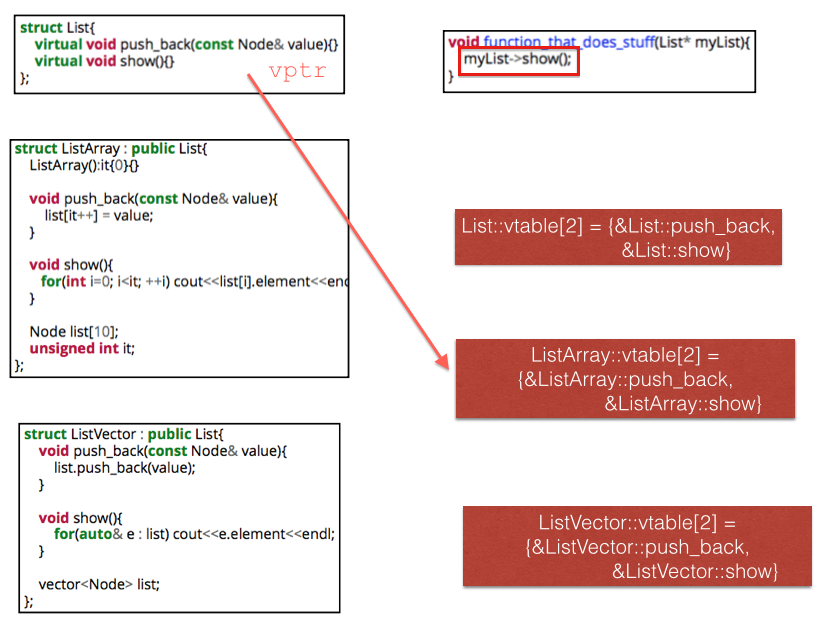
\includegraphics[height=70mm]{/Users/lalanne/MyCode/GitHubProjects/MetaTalk/figures/vtblpluscall4.png}\hspace{5mm}
            };
        \end{tikzpicture}
    \end{center}
\end{frame}

\begin{frame}{Virtual Functions}
    \begin{center}
        \begin{tikzpicture}[]
            \node[] at (0mm,0mm){
                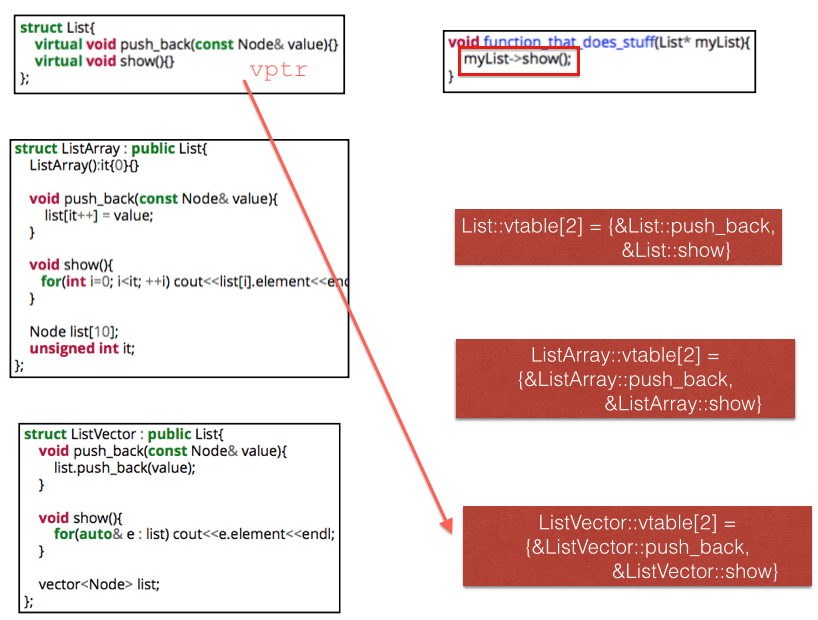
\includegraphics[height=70mm]{/Users/lalanne/MyCode/GitHubProjects/MetaTalk/figures/vtblpluscall5.png}\hspace{5mm}
            };
        \end{tikzpicture}
    \end{center}
\end{frame}

\begin{frame}{Virtual Functions}
    \begin{itemize}
        \item First load \emph{vptr} to register (r1)
        \item Second load \emph{vptr + offset} to register (r2)
        \item Call function (r2)
    \end{itemize}

    \begin{itemize}
        \item Small size overhead(think small classes)
        \item Call overhead
    \end{itemize}
\end{frame}

